% Settings for the default beamer theme
\documentclass[english, aspectratio=169]{beamer}
\usepackage{babel}
\usepackage{tabularx}
\usepackage[T1]{fontenc}
\usepackage[utf8]{inputenc}
\usepackage[ruled,vlined]{algorithm2e}
\SetAlgorithmName{Algoritmus}{algoritmus}{List of Algorithms}
\setcounter{secnumdepth}{3}
\setcounter{tocdepth}{3}

\makeatletter

\newcommand\makebeamertitle{\frame{\maketitle}}

% (ERT) argument for the TOC
\AtBeginDocument{%
  \let\origtableofcontents=\tableofcontents
  \def\tableofcontents{\@ifnextchar[{\origtableofcontents}{\gobbletableofcontents}}
  \def\gobbletableofcontents#1{\origtableofcontents}
}

% Theme settings
\usetheme{Frankfurt}
\usecolortheme{default}
\usefonttheme[onlymath]{serif}

% Template settings
\setbeamertemplate{navigation symbols}{}
\setbeamertemplate{blocks}[rounded][shadow=false]
\setbeamertemplate{title page}[default][colsep=-4bp, rounded=true, shadow=false]
\makeatother

\begin{document}

% Title page
\section{Bevezetés}
\title[]{Üzleti Intelligencia}
\subtitle{3. Előadás: Markov döntési folyamatok megoldása}
\author[Kuknyó Dániel]{Kuknyó Dániel\\Budapesti Gazdasági Egyetem}
\date{2023/24\\1.félév}
\makebeamertitle

% Table of contents slide
\begin{frame}
\tableofcontents{}
\end{frame}

% Table of contents of the current section
\begin{frame}
\tableofcontents[currentsection]
\end{frame}

\begin{frame}{Az RL modellje}
\begin{columns}
\begin{column}{.5\textwidth}
\only<1>{\begin{block}{Markov döntési folyamat}
\[
MDP\left(S,A,P,R,s_{0},\gamma\right)
\]
\begin{itemize}
	\item $S$: állapotok halmaza
	\item $A$: cselekvések halmaza
	\item $P:\; S \times A \times S \rightarrow [0,1]$: állapotátmeneti valószínűségek
	\item $R:\; S \times A \rightarrow \mathbb{R}$: azonnali jutalmak
	\item $s_{0}$: kezdőállapot
	\item $\gamma$: diszkont faktor
\end{itemize}
\end{block}}
\only<2>{Az MDP folyamata:\\
\begin{enumerate}
	\item Az ügynök $s_{0}$ állapotból indul
	\item Az ügynök $\pi$ politika szerint cselekszik: $a_{t}\sim\pi(s_{t})$
	\item A környezet reagál a cselekvésre, és visszaadja az ügynöknek $r_{t+1}$ jutalmat és $s_{t+1}$ következő állapotot
	\item Ez ismétlődik amíg a kilépési kritérium be nem teljesül
\end{enumerate}
Cél: Az optimális politika megtalálása. A politika optimális, ha a hozamának várható értéke maximális:
\[
E_{\pi}\left(r_{1} + \gamma r_{2} + \gamma^{2}r_{3} + ...\right) \rightarrow max
\]}
\end{column}
\begin{column}{.5\textwidth}
\begin{center}
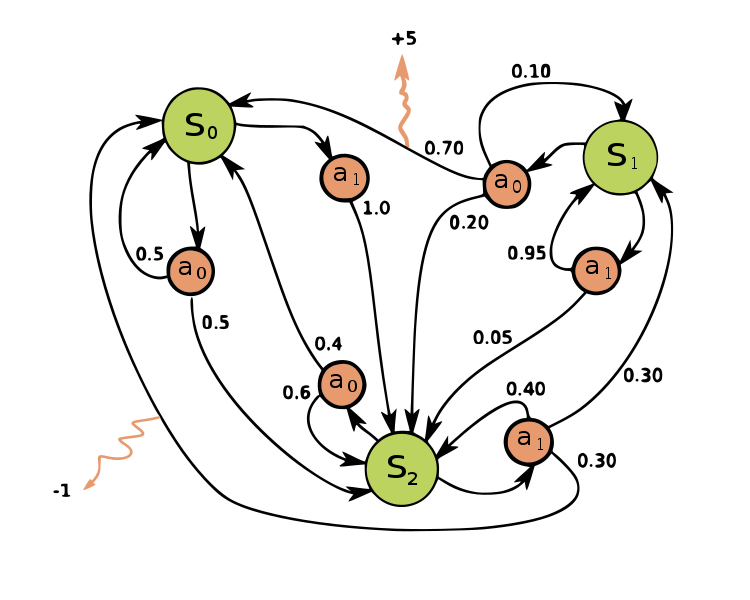
\includegraphics[width=7cm, height=7cm, keepaspectratio]{images/solving_1.png}
\end{center}
\end{column}
\end{columns}
\end{frame}

\begin{frame}{A mohó ügynök}
\begin{columns}[T]
\begin{column}{.5\textwidth}
A legegyszerűbb cselekvés kiválasztási szabály, ha az ügynök mindig azt a cselekvést választja, ami számára a lehető legnagyobb várható hozammal rendelkezik.
\begin{center}
\begin{block}{Mohó cselekvés választás}
Mohó politika mindig azt a cselekvést fogja választani, amelyik - egy lépéses távlatban - a lehető legnagyobb várható jutalommal fog járni az ügynök számára $v_{\pi}$ szerint.
\[
A_{t}=\underset{a}{argmax}\:Q_{t}(a)
\]
\end{block}
\end{center}
\end{column}
\begin{column}{.5\textwidth}
\begin{itemize}
	\item Mi lenne a mohó politika ebben az estben?
	\item Mindig ez a legjobb megoldás?
	\item A legjobb megoldás mindig mohó?
\end{itemize}
\begin{center}
\only<1>{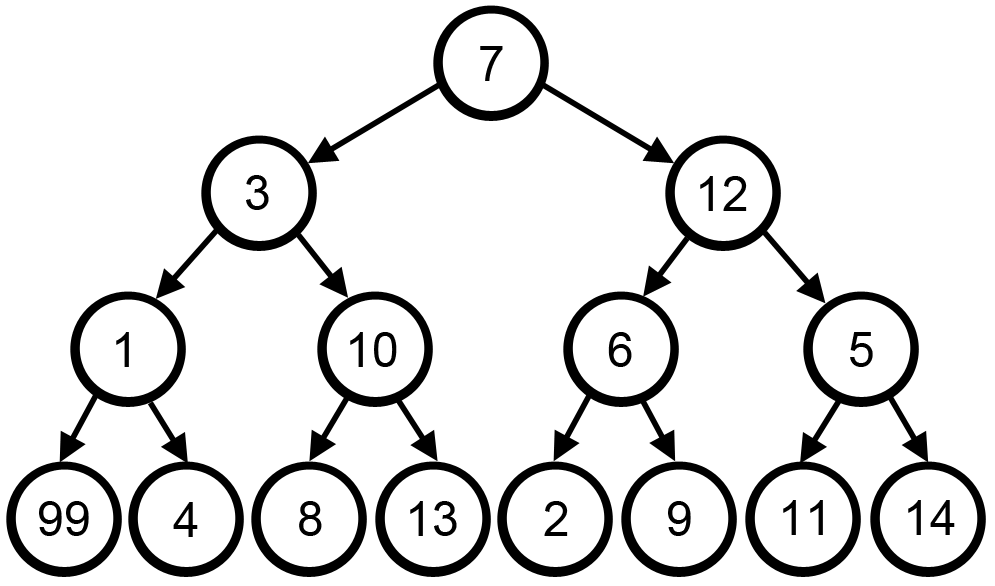
\includegraphics[width=7cm, height=7cm, keepaspectratio]{images/solving_2.png}}
\only<2>{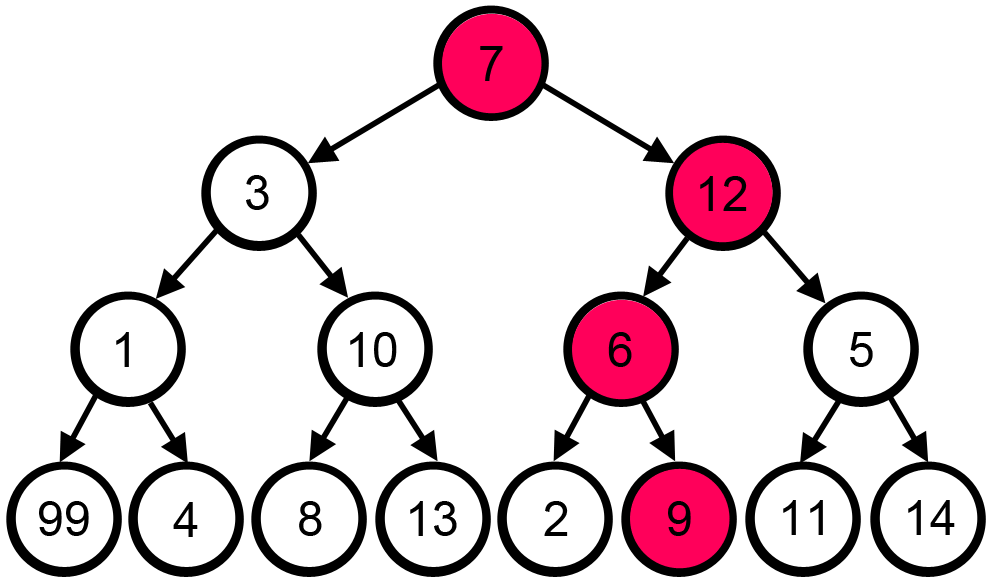
\includegraphics[width=7cm, height=7cm, keepaspectratio]{images/solving_3.png}}
\end{center}
\end{column}
\end{columns}
\end{frame}

\begin{frame}{Az $\varepsilon$-mohó stratégia}
\begin{columns}
\begin{column}{.5\textwidth}
Egy másik lehetőség, ha adott valószínűséggel az ügynök véletlen cselekvést hajt végre remélve, hogy ezzel elér egy olyan állapotba amelyhez nagy jutalom tartozik. A véletlen cselekvés a \textbf{felfedezés}, és végrehajtásának valószínűsége $\epsilon$.
\begin{center}
\begin{block}{$\varepsilon$-mohó cselekvés választás}
\[
A_{t}\leftarrow\begin{cases}
_{a\sim A}^{\underset{a}{argmax}Q(a)} & _{P=\varepsilon}^{P=1-\varepsilon}\end{cases}
\]
\end{block}
\end{center}
\end{column}
\begin{column}{.5\textwidth}
Az ügynök tehát $\varepsilon$ valószínűséggel véletlen cselekvést választ az ismeretlen, de nagyobb jutalom reményében. Ez a \textbf{felfedezés} művelete.\\
$\varepsilon$ valószínűséggel pedig a már ismert és a legnagyobb várható jutalommal járó cselekvést hajtja végre. Ez a \textbf{kizsákmányolás} művelete.
\begin{center}
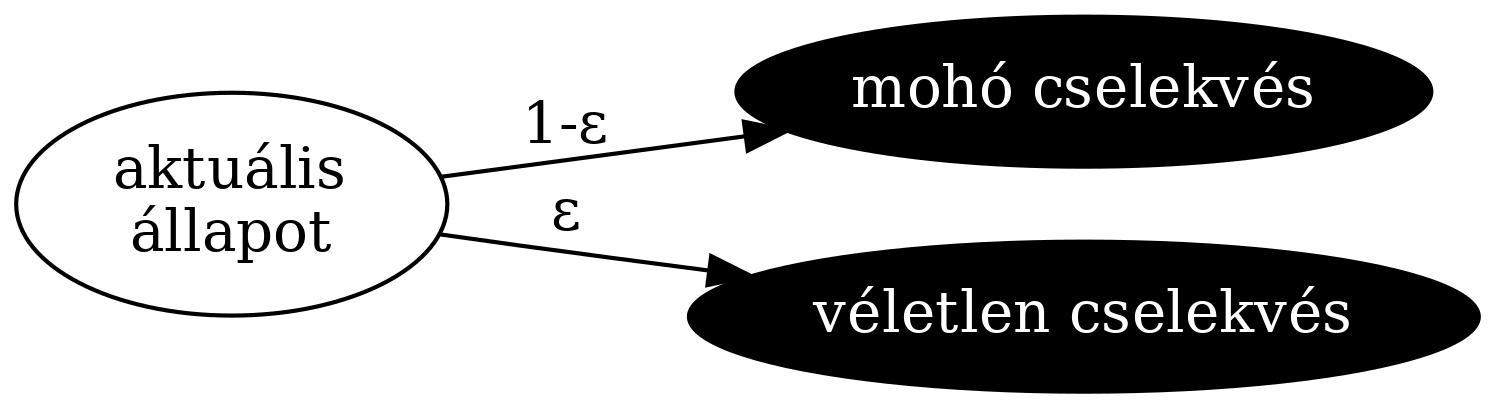
\includegraphics[width=7cm, height=6cm, keepaspectratio]{graphs/solving_1.png}
\end{center}
\end{column}
\end{columns}
\end{frame}

\begin{frame}{Példák}
A következő valós példák alkalmasak a felfedezés/kizsákmányolás dilemma bemutatására:
\begin{itemize}
	\item Étterem választás:
	\begin{itemize}
		\item \textbf{Kizsákmányolás}: elmész a kedvenc éttermedbe.
		\item \textbf{Felfedezés}: elmész egy új étterembe, hátha találsz egy jobbat mint a kedvenced.
	\end{itemize}
	\item Online hirdetés:
	\begin{itemize}
		\item \textbf{Kizsákmányolás}: a legjobb reklám megmutatása a felhasználónak.
		\item \textbf{Felfedezés}: egy új reklám megmutatása a felhasználónak, hátha tetszik neki.
	\end{itemize}
	\item Olajfúrás:
	\begin{itemize}
		\item \textbf{Kizsákmányolás}: Egy meglévő helyen fúrás az olajért.
		\item \textbf{Felfedezés}: Egy új helyen fúrás.
	\end{itemize}
	\item Klinikai kezelés:
	\begin{itemize}
		\item \textbf{Kizsákmányolás}: A bevált kezelés alkalmazása.
		\item \textbf{Felfedezés}: Új kezelés kipróbálása.
	\end{itemize}
\end{itemize}
\end{frame}

\section{A rabló probléma}

\begin{frame}
\tableofcontents[currentsection]
\end{frame}

\begin{frame}{A rabló probléma}
\begin{columns}
\begin{column}{.5\textwidth}
\only<1>{A $k$-karú rabló problémája egy elméleti megerősítéses tanulás probléma. A játékos egy rablógépen játszik, amelynek $k$ karja van. \\
Minden karhúzás után egy állandó eloszlásból választott jutalmat kap az ügynök. Az ügynök célja, hogy olyan politikát válasszon, ami az elvárt hozamot maximalizálja $1000$ cselekvés vagy \emph{időlépés} után.}
\only<2>{Az ügynöknek számon kell tartania, mennyi a jutalom várható értéke, ha adott egy $a$ cselekvés. Ez a $Q(s,a)$ állapot-cselekvés minőség függvény. A rabló problémában csak egy állapot van, ezért elég csak a cselekvésekhez tartozóan számon tartani:
\begin{block}{}
\[
q_{*}(a)=E\left[r_{t}|A_{t}=a\right]
\]
\end{block}
A jutalom várható értéke: 
\begin{block}{}
\[
Q_{n}=\frac{r_{1}+r_{2}+...+r_{n-1}}{n-1}
\]
\end{block}
}
\end{column}
\begin{column}{.5\textwidth}
\begin{center}
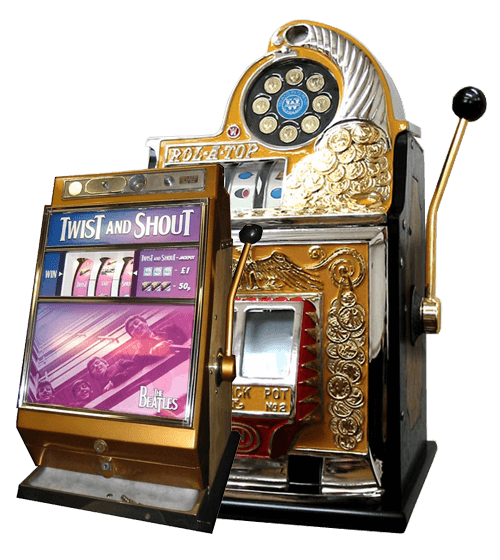
\includegraphics[width=7cm, height=7cm, keepaspectratio]{images/solving_5.png}
\end{center}
\end{column}
\end{columns}
\end{frame}

\begin{frame}{A rabló folyamat modellje}
\begin{columns}
\begin{column}{.5\textwidth}
A példában egy kétkarú rabló folyamat modellje látható. A modell egyetlen állapotot tartalmaz. az ügynök minden lépésben innen választhat, hogy melyik kart húzza meg. Ez a két cselekvéssel egyezik meg: $a_{1}, a_{2}$.\par\smallskip
A jutalmak minden cselekvés után egy normál eloszlásból származnak, valamilyen $\mu_{1}$ és $\mu_{2}$ várható értékkel és $1$ szórással: $r\sim N(\mu_{1},1)$.
\end{column}
\begin{column}{.5\textwidth}
\begin{center}
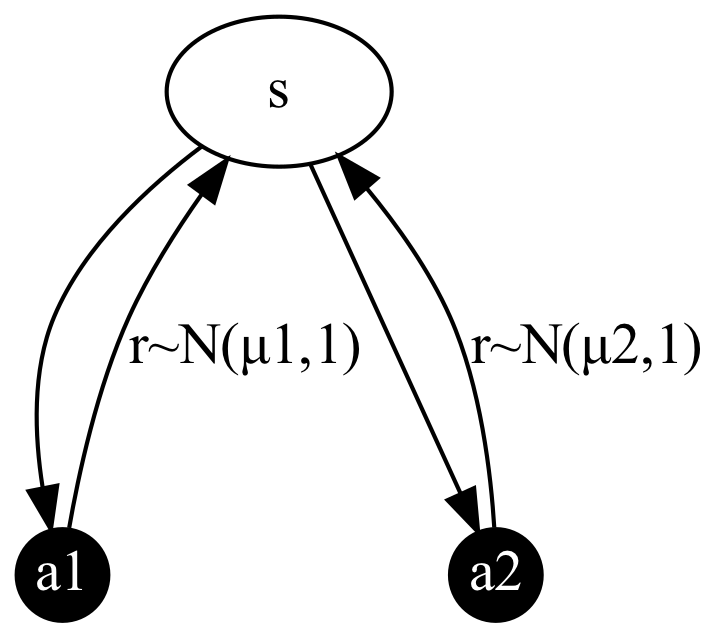
\includegraphics[width=7cm, keepaspectratio]{graphs/solving_0.png}
\end{center}
\end{column}
\end{columns}
\end{frame}

\begin{frame}
\begin{algorithm}[H]
\caption{Rabló játék}
\SetAlgoLined
	$Q(a)\leftarrow0$ \textbf{for} $a=1\rightarrow k$\tcc*[r]{Cselekvés minőségének függvénye}
	$N(a)\leftarrow	0$ \textbf{for} $a=1\rightarrow k$\tcc*[r]{Kar meghúzásainak a száma}
	\For{$t=1 \rightarrow max_{t}$}{
		$p=random(0,1)$\tcc*[t]{Véletlen szám $0$ és $1$ között}
		\eIf{$p>\varepsilon$}{
			$a \leftarrow \underset{a}{argmax}Q(a)$\tcc*[r]{Legnagyobb ismert jutalom cselekvése}
		}{
			$a \leftarrow a \sim A $\tcc*[r]{Véletlen cselekvés}
		}
		$r\leftarrow env(a)$\tcc*[t]{Cselekvés végrehajtása a környezetben}
		$N(a) \leftarrow N(a)+1$\tcc*[t]{Cselekvés számlálójának növelése}
		$Q(a) \leftarrow Q(a) + \frac{1}{N(a)}\left[r-Q(a)\right]$\tcc*[t]{$Q$-érték frissítése}
	}
\end{algorithm}
\end{frame}

\begin{frame}{Egy példa rabló}
\begin{columns}
\begin{column}{.5\textwidth}
Hogy meg lehessen mérni a mohó és $\varepsilon$-mohó stratégiák teljesítményét, szükség van egy teszt rablóra. A példában szereplő egy $10$-karú rabló. Minden karhoz tartozóan a jutalmak eloszlása Gauss-i eloszlást követ $1$ varianciával, viszont nem $0$ átlaggal. \par\smallskip
Valamelyik karok nagyobb valószínűséggel járnak magas jutalommal mint a többi. Az ügynök feladata megtalálni melyik kartól remélhet nagyobb jutalmat. Ehhez szükség van arra, hogy végig próbálja őket.
\end{column}
\begin{column}{.5\textwidth}
\begin{center}
A jutalmak eloszlása
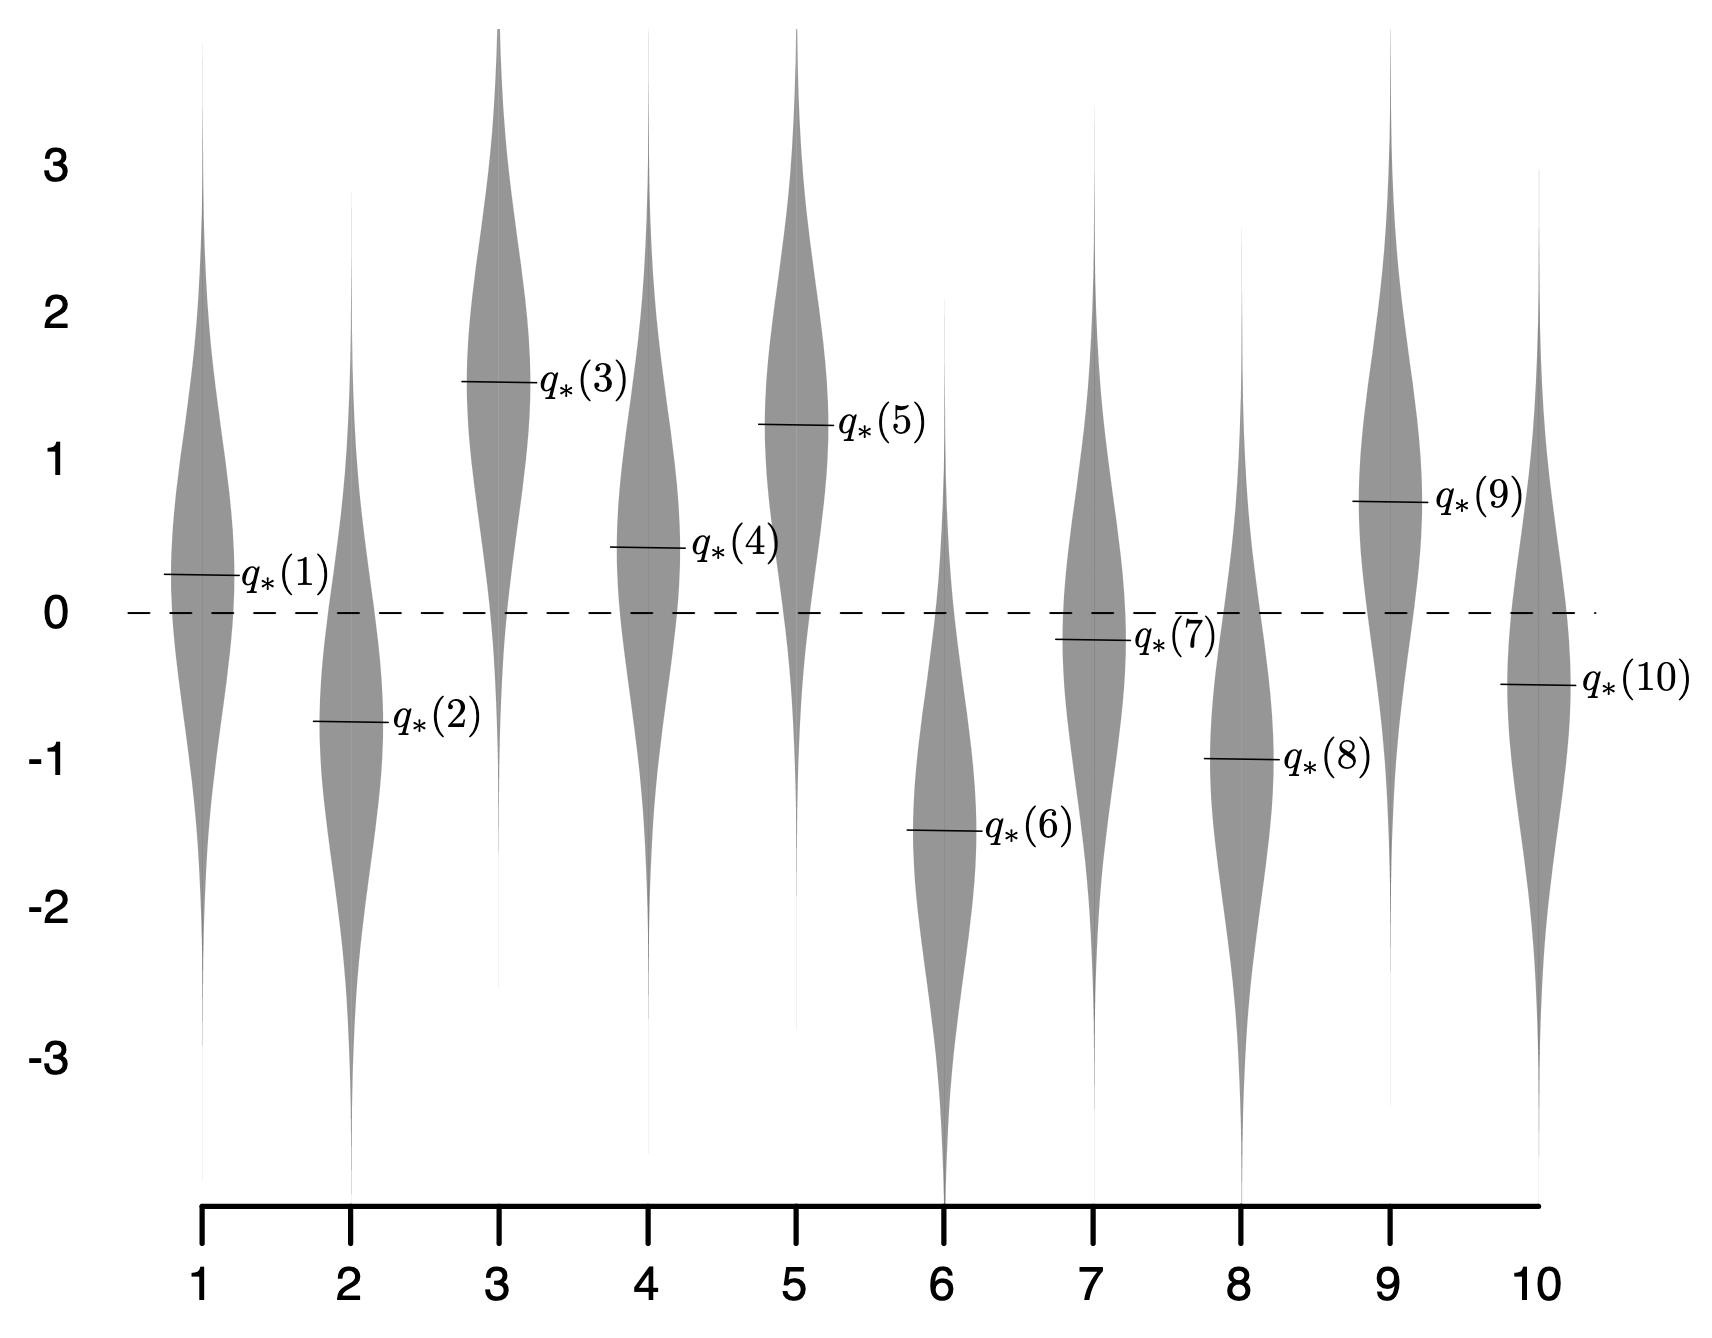
\includegraphics[width=7cm, height=6cm, keepaspectratio]{images/solving_6.png}
\begin{scriptsize}
Cselekvés
\end{scriptsize}
\end{center}
\end{column}
\end{columns}
\end{frame}

\begin{frame}{A futás teljesítménye}
\begin{columns}
\begin{column}{.5\textwidth}
Az algoritmus $1000$ időlépésen keresztül futott $\varepsilon=0,\varepsilon=0.01,\varepsilon=0.001$ hiperparaméterekkel. Minél nagyobb a $\varepsilon$ érték, annál nagyobb a felfedezés valószínűsége. \par\smallskip 
Mindegyik módszer megbecsülte az állapot-cselekvés minőség függvényt a rabló minden karára a mozgóátlagolás technikájával. A diagramon a várható jutalom mértékét mutatja az időlépések függvényében. 
\par\smallskip
A mohó stratégia kezdetben gyorsabban javult mint a többi, de kisebb értékre konvergált a futásidő végére.
\end{column}
\begin{column}{.5\textwidth}
\begin{center}
Átlagos jutalom
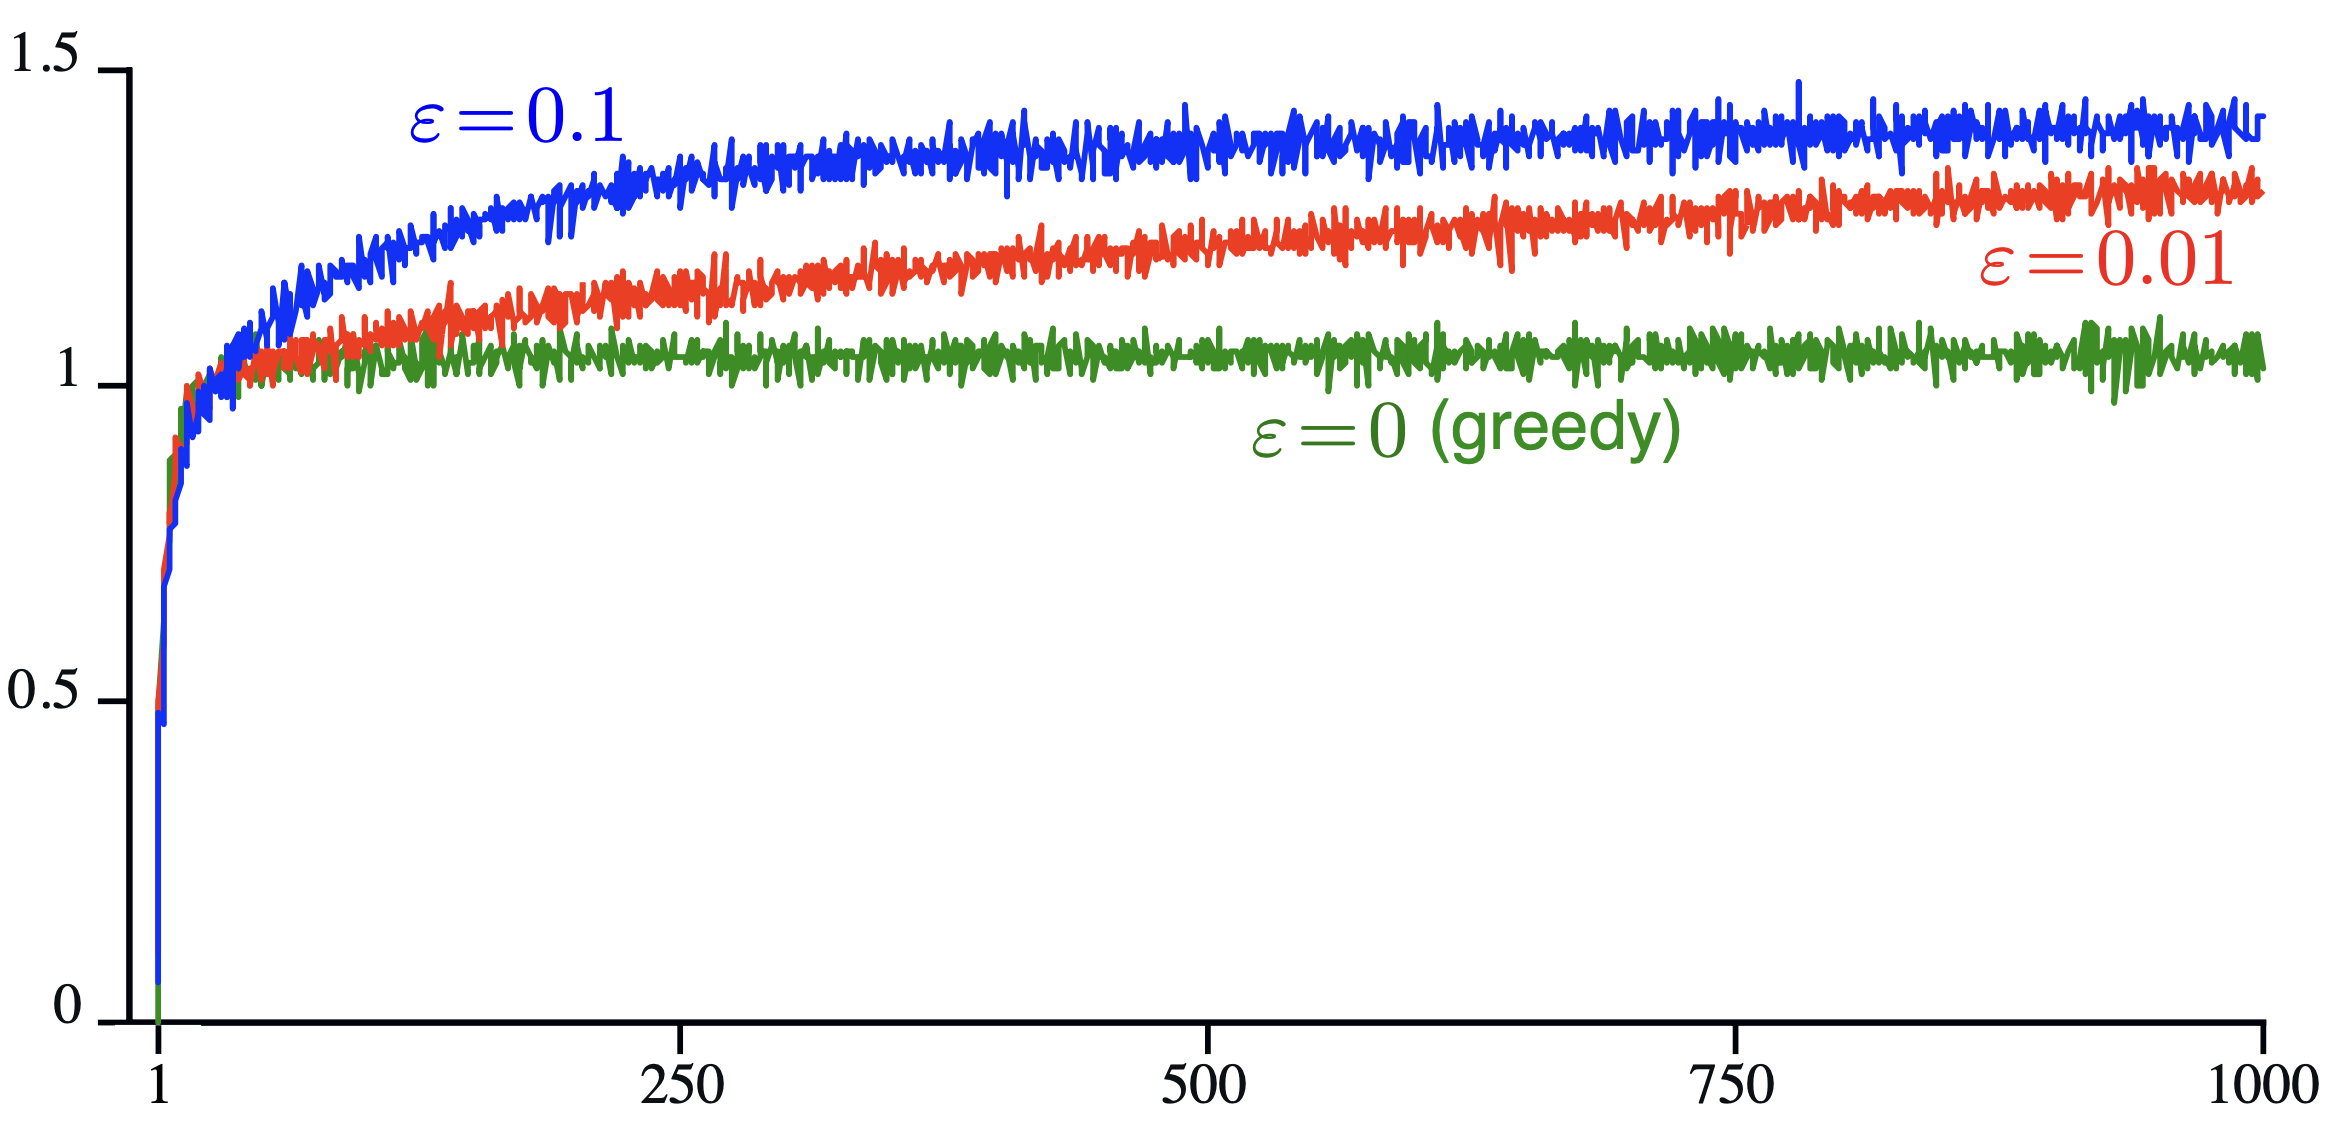
\includegraphics[width=7cm, keepaspectratio]{images/solving_7.png}
\begin{scriptsize}
Időlépés
\end{scriptsize}
\end{center}
\end{column}
\end{columns}
\end{frame}

\begin{frame}{A futás teljesítménye}
\begin{columns}
\begin{column}{.5\textwidth}
Az ábra azt mutatja, hogy a mohó módszer csak a feladatok mintegy $30\%$-ában találta meg az optimális műveletet. Az $\varepsilon$-mohó módszerek végül jobban teljesítettek, mert folytatták a felfedezést és javították az esélyüket az optimális művelet felismerésére. \par\smallskip
Az $\varepsilon=0.1$ módszer többet fedezett fel, és általában korábban megtalálta az optimális műveletet, de soha nem választotta ki azt több mint $91\%$-ban. \par\smallskip
Az $\varepsilon=0.01$ módszer lassabban javult, de végül mindkét teljesítménymérőn jobban teljesített.
\end{column}
\begin{column}{.5\textwidth}
\begin{center}
Optimális cselekvés aránya
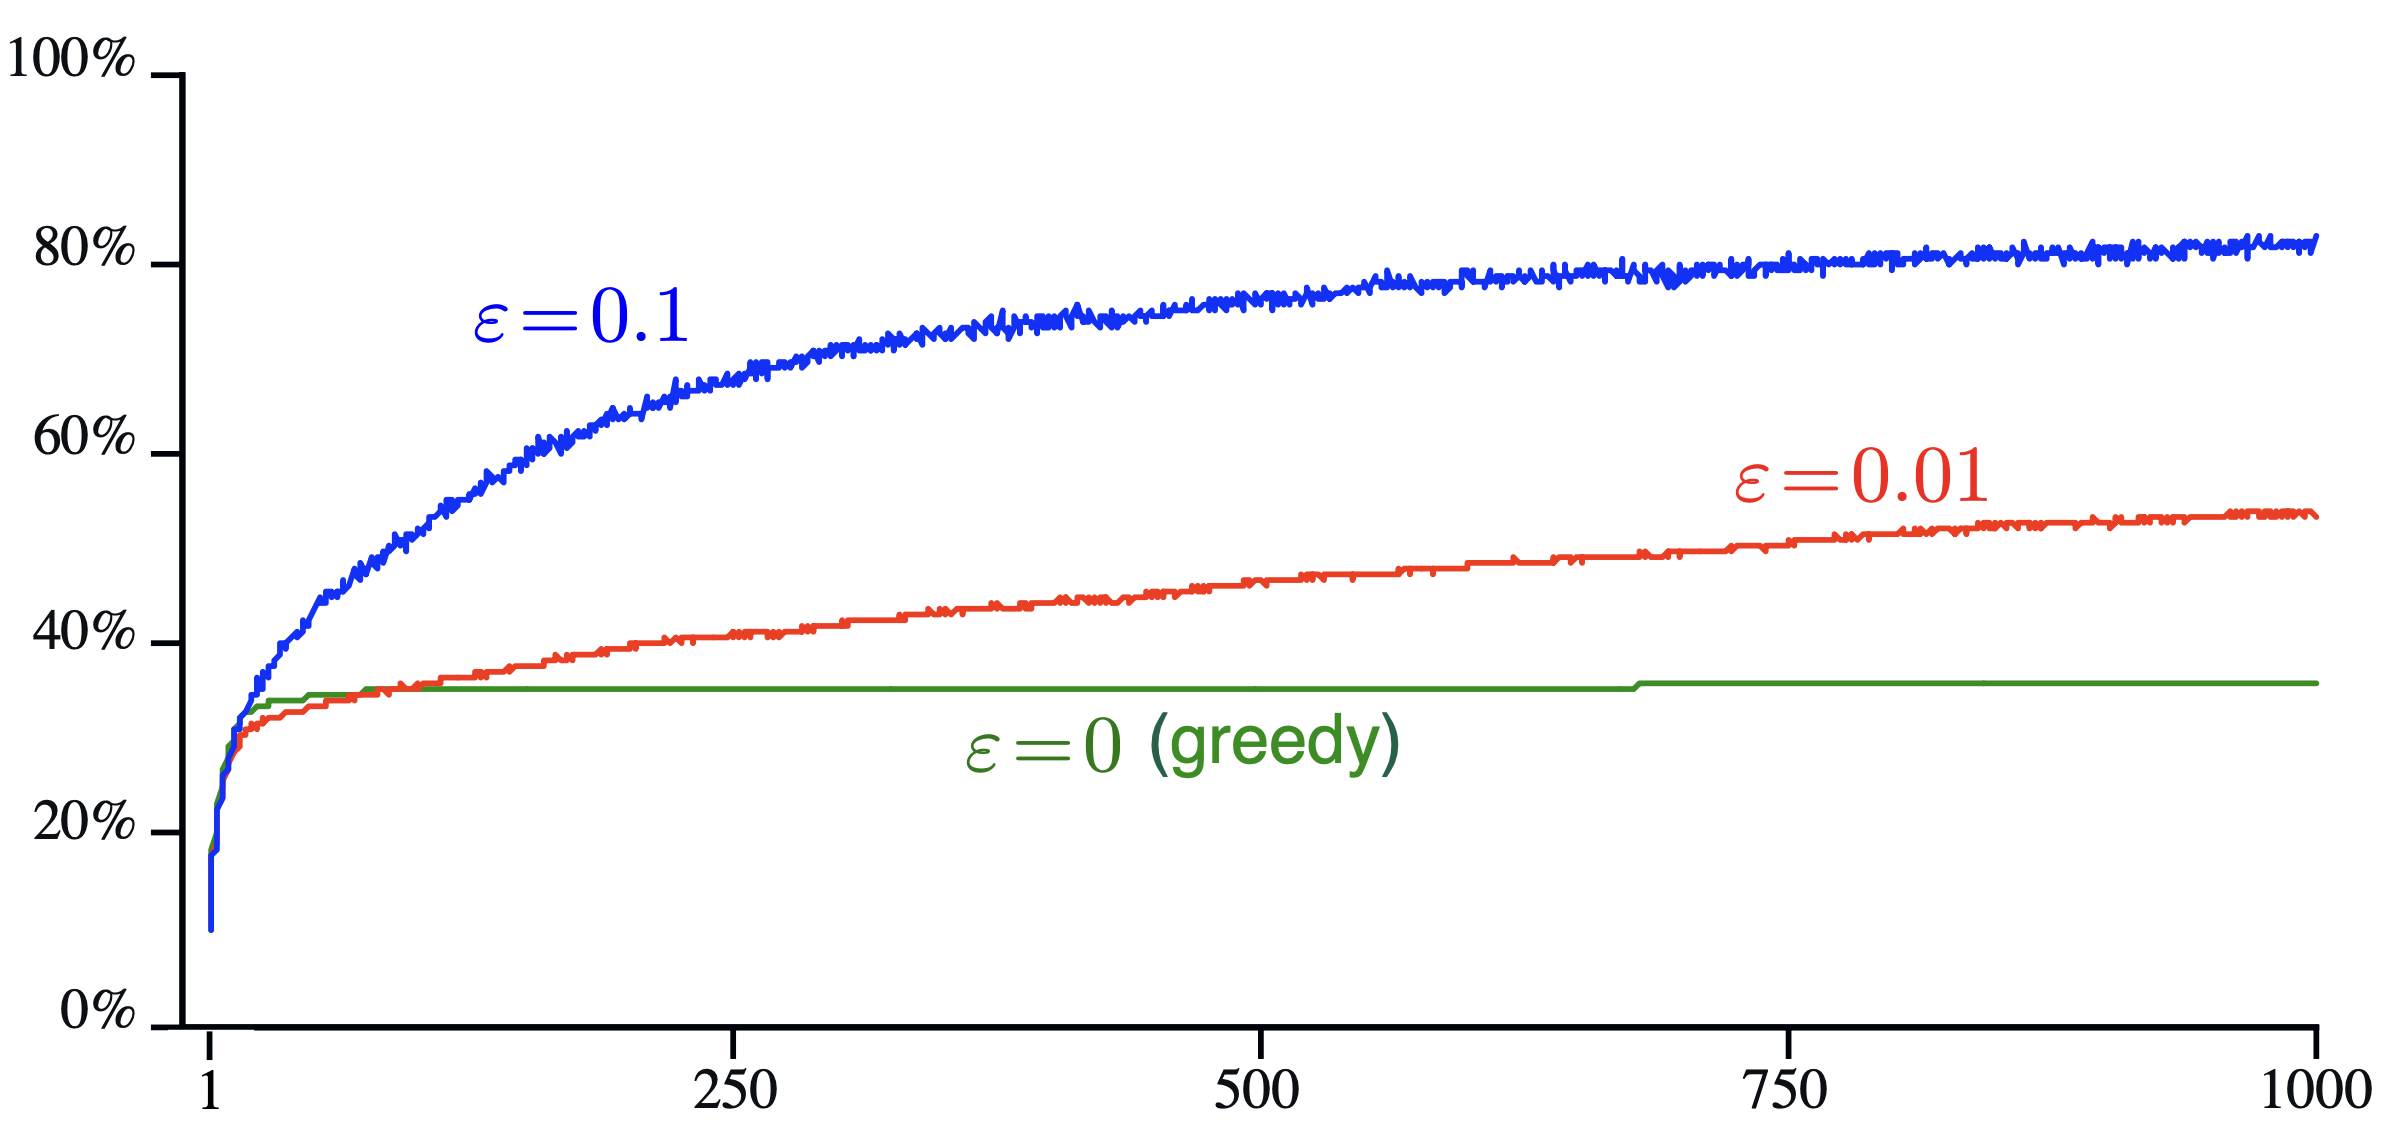
\includegraphics[width=7cm, keepaspectratio]{images/solving_8.png}
\begin{scriptsize}
Időlépés
\end{scriptsize}
\end{center}
\end{column}
\end{columns}
\end{frame}

\section{Dinamikus programozás}

\begin{frame}
\tableofcontents[currentsection]
\end{frame}

\begin{frame}{Dinamikus programozás alapjai}
\begin{columns}
\begin{column}{.5\textwidth}
\only<1>{A dinamikus programozás egy gyűjtőfogalom olyan algoritmusokra amelyekkel kiszámolható az optimális politika \emph{ha adott egy tökéletes környezeti modell egy Markov döntési folyamatként}.\par\smallskip
A klasszikus dinamikus programozási algoritmusok ritkák a megerősítéses tanulásban mert egy tökéletes környezeti modellt feltételeznek és mert rendkívül erőforrás igényesek.}
\only<2>{\begin{center}
\begin{block}{Dinamikus programozás}
A DP algoritmusok a komplex problémákat alproblémákra bontják, majd a végső megoldást az alproblémák megoldásaiból állítják elő. Ehhez két feltételnek kell érvényesnek lennie:
\begin{itemize}
	\item \textbf{Optimális alstruktúra}: Az almegoldásoknak felhasználhatóknak kell lenniük a probléma megoldására.
	\item \textbf{Átfedésben lévő alproblémák}: Bizonyos alproblémák megoldásait többször is fel lehet használni hasonló feladatok elvégzéséhez.
\end{itemize}
\end{block}
\end{center}}
\end{column}
\begin{column}{.5\textwidth}
\begin{center}
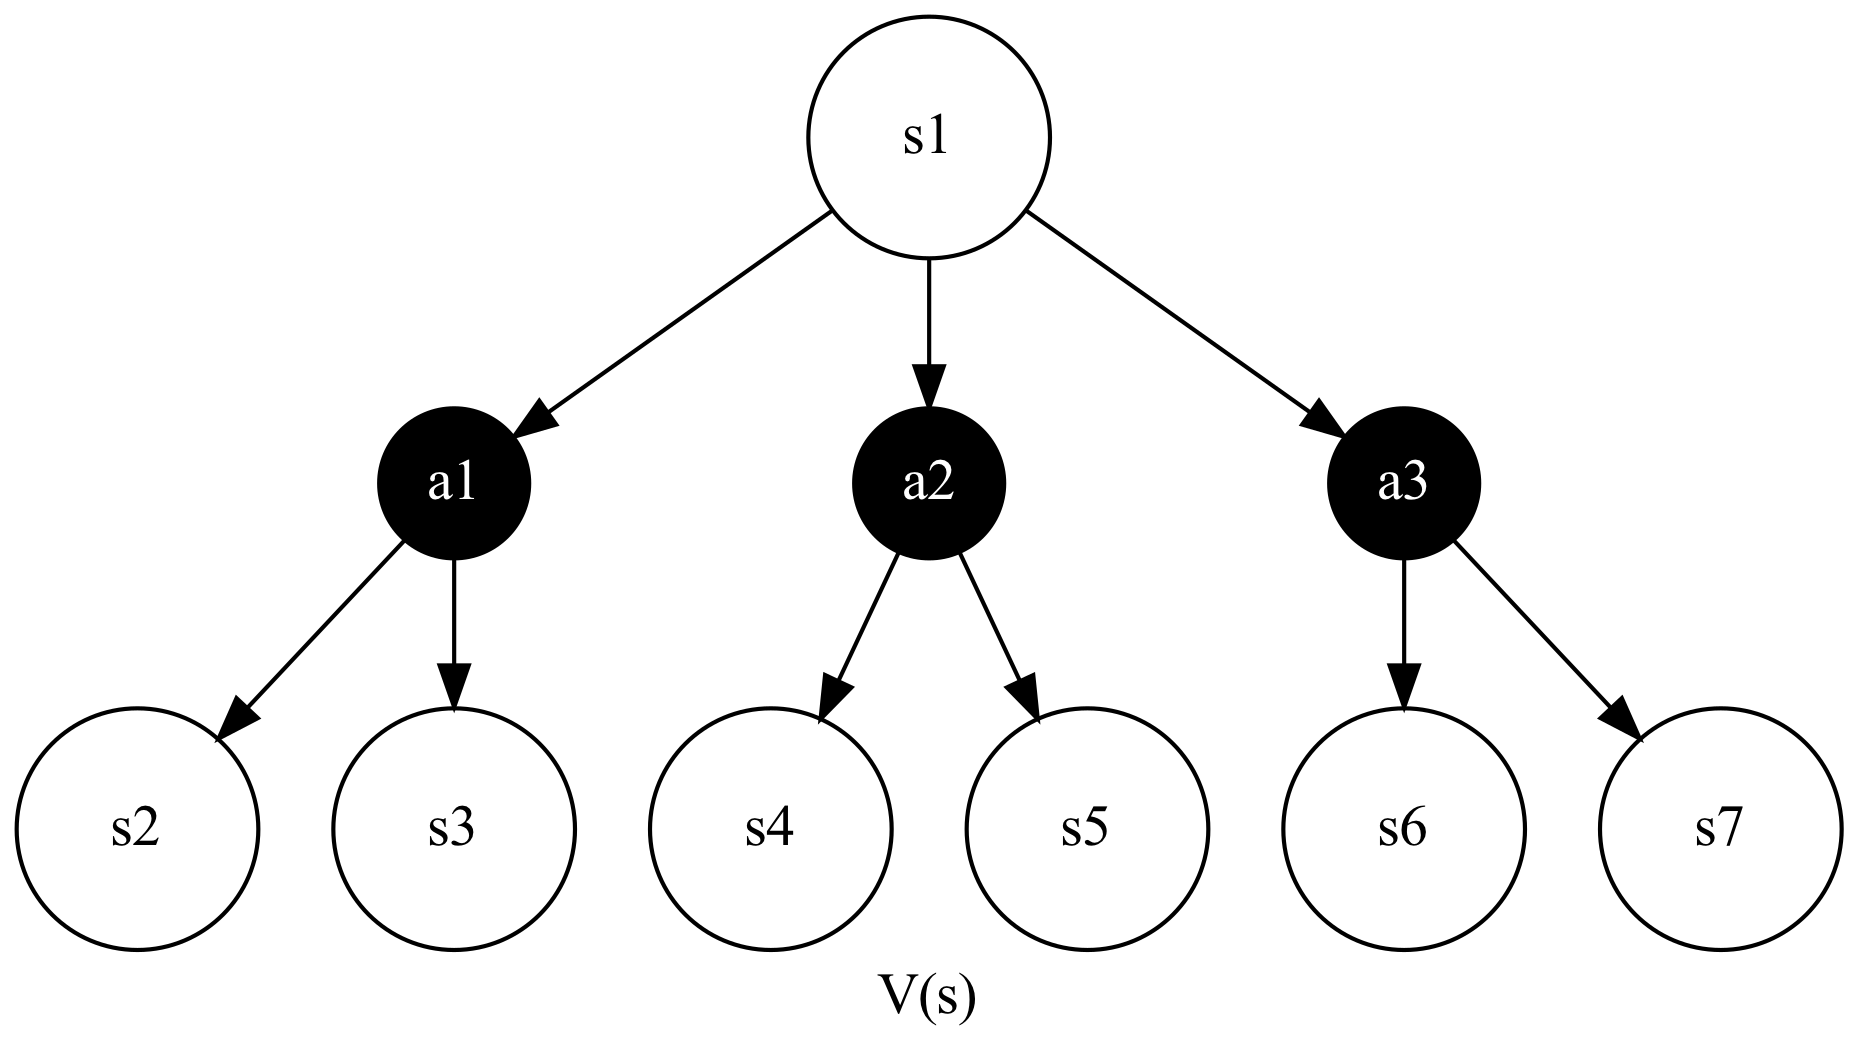
\includegraphics[width=7cm, keepaspectratio]{graphs/solving_5.png}
\end{center}
\end{column}
\end{columns}
\end{frame}

\begin{frame}{Példa dinamikus programozásra}
\begin{columns}
\begin{column}{.5\textwidth}
A példa a Fibonacci számok kiszámításának dinamikus programozása. A Fibonacci számokat a következőképpen lehet definiálni:\\
\begin{block}{Fibonacci sorozat}
\[
F_{0}=0\;;F_{1}=1
\]
és
\[
F_{n}=F_{n-1}+F_{n-2}
\]
\end{block}
Tehát a sorozat első pár tagja:
\[
0, 1, 1, 2, 3, 5, 8, 13, 21, 34, 55, 89, 144
\]
\end{column}
\begin{column}{.5\textwidth}
\begin{center}
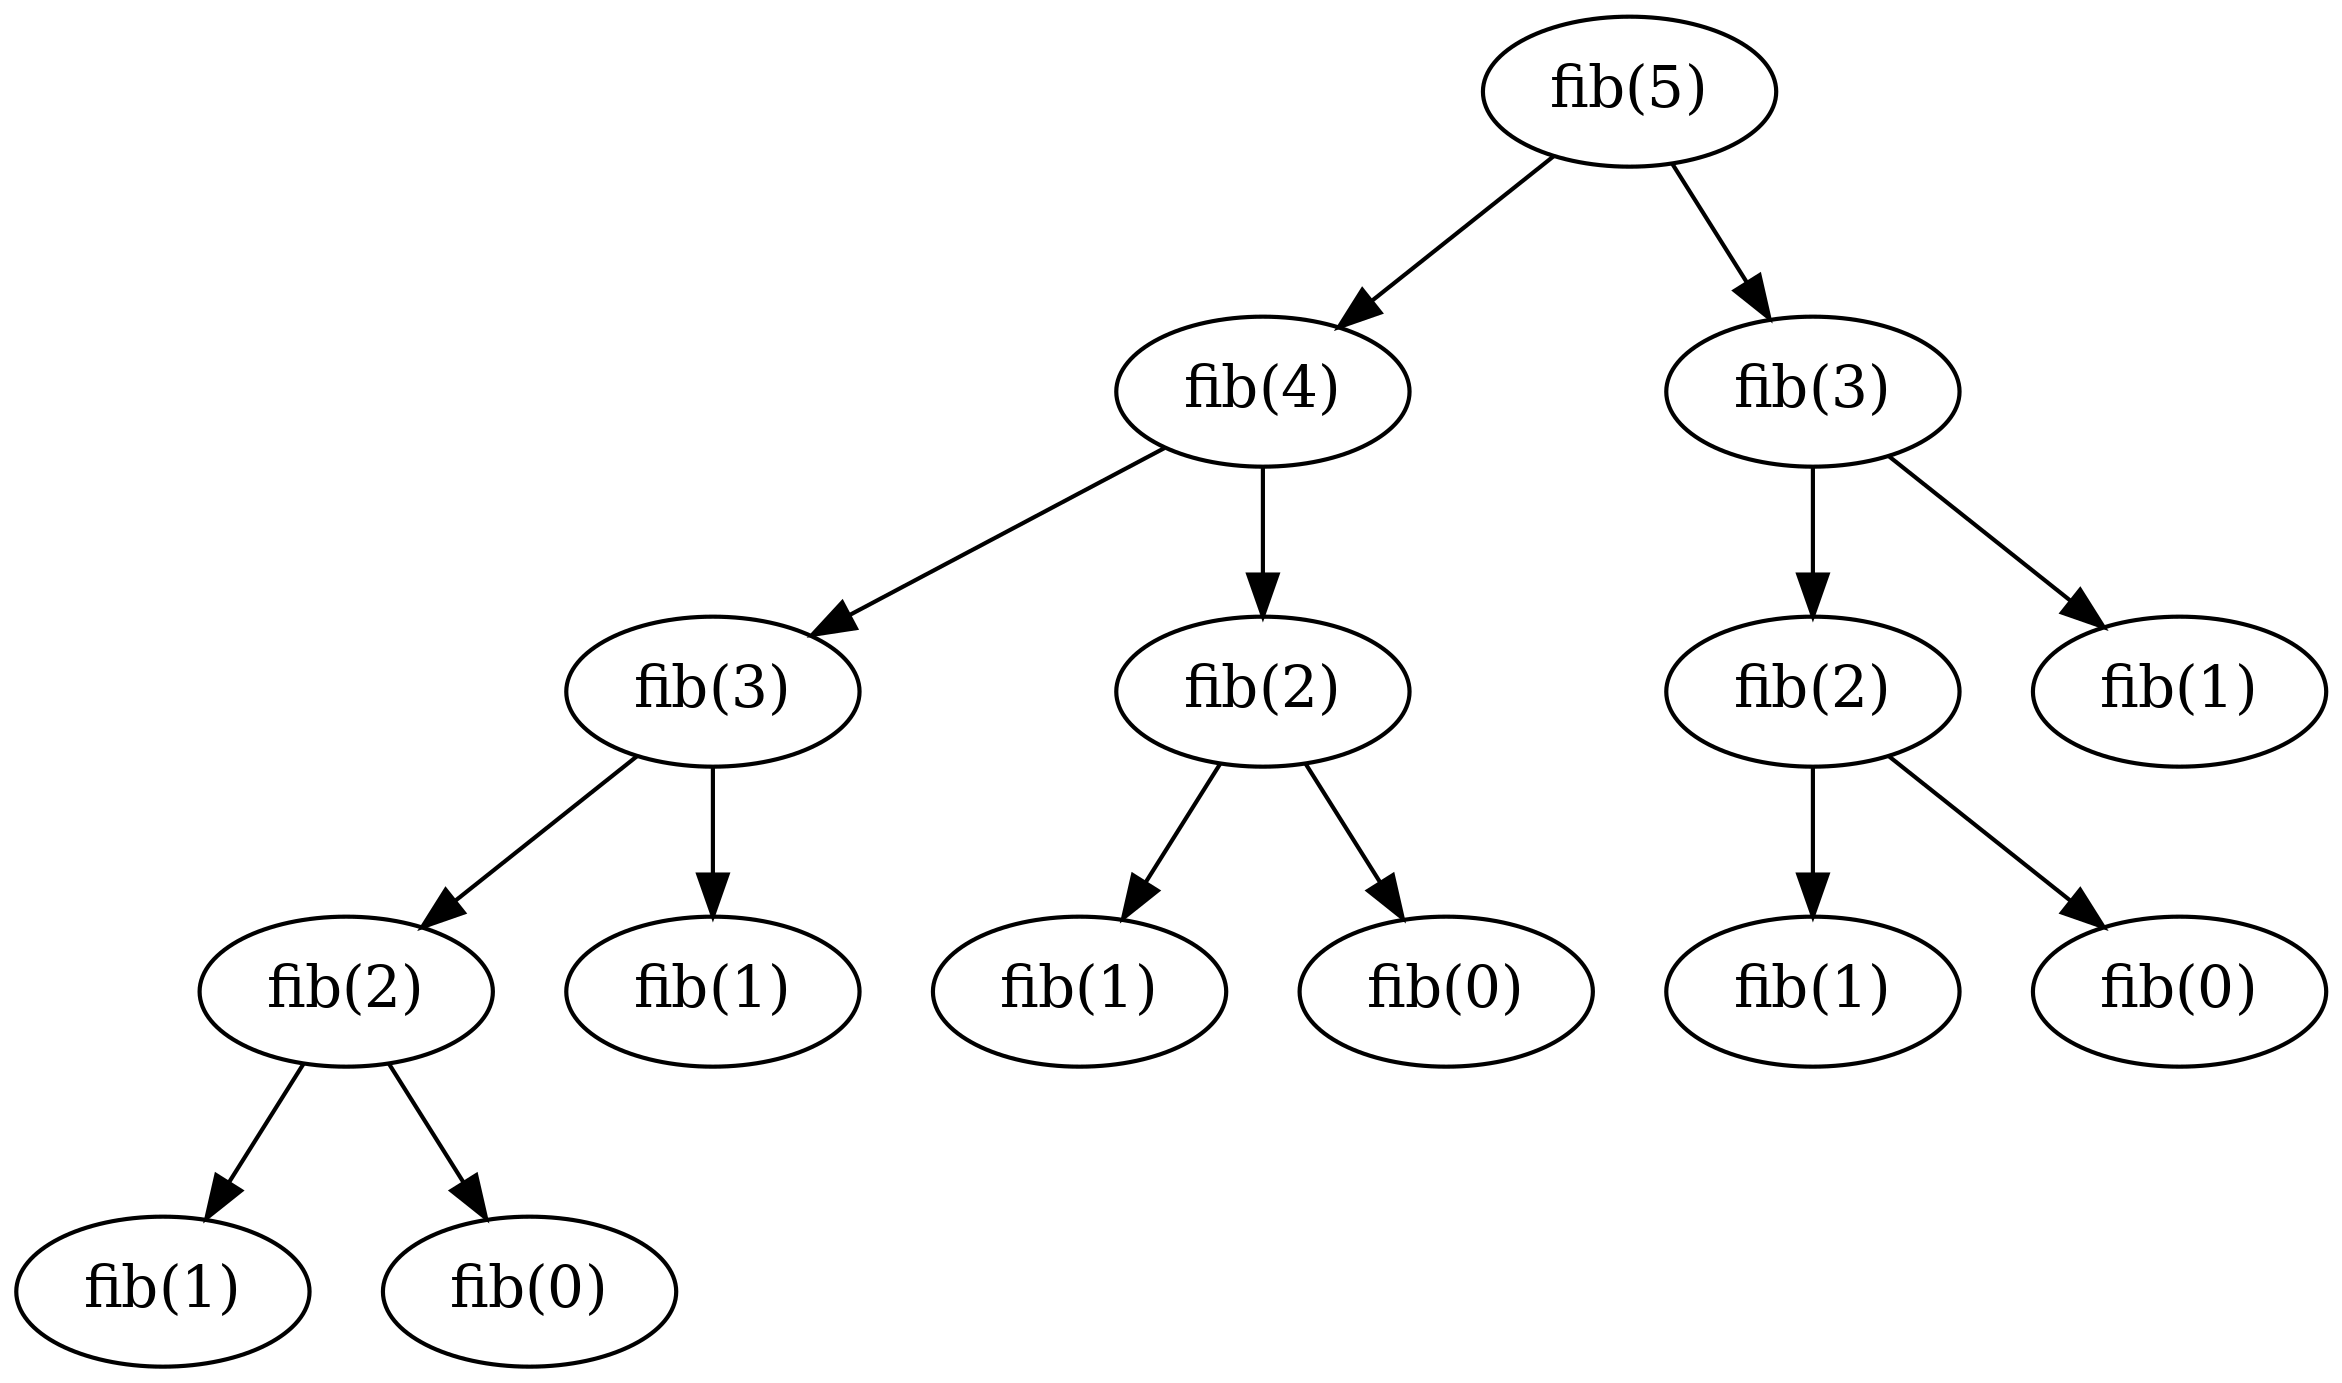
\includegraphics[width=7cm, keepaspectratio]{graphs/solving_4.png}
\end{center}
\end{column}
\end{columns}
\end{frame}

\begin{frame}{Dinamikus programozás az RL-ben}
\begin{columns}
\begin{column}{.5\textwidth}
\begin{block}{DP állapot-érték frissítési szabálya}
\[
V(s_{t})\leftarrow E_{\pi}\left[r_{t+1} + \gamma V(s_{t+1})\right]
\]
\begin{itemize}
	\item $E_{\pi}$: várható érték $\pi$ politika alatt
	\item $V(s_{t})$: cselekvés-érték függvény az aktuális $s$ állapotban
	\item $r_{t+1}$: a jutalom a következő cselekvésért
	\item $\gamma$: diszkont faktor
	\item $V(s_{t+1})$ vagy $s'$: cselekvés-érték függvény a következő állapotban.
\end{itemize}
\end{block}
\end{column}
\begin{column}{.5\textwidth}
A megerősítéses tanulásban a dinamikus programozás egy szélességi bejárásnak felel meg. Mivel az állapotok tere túlságosan nagy, ez gyakran nem vezet megoldáshoz. 
\begin{center}
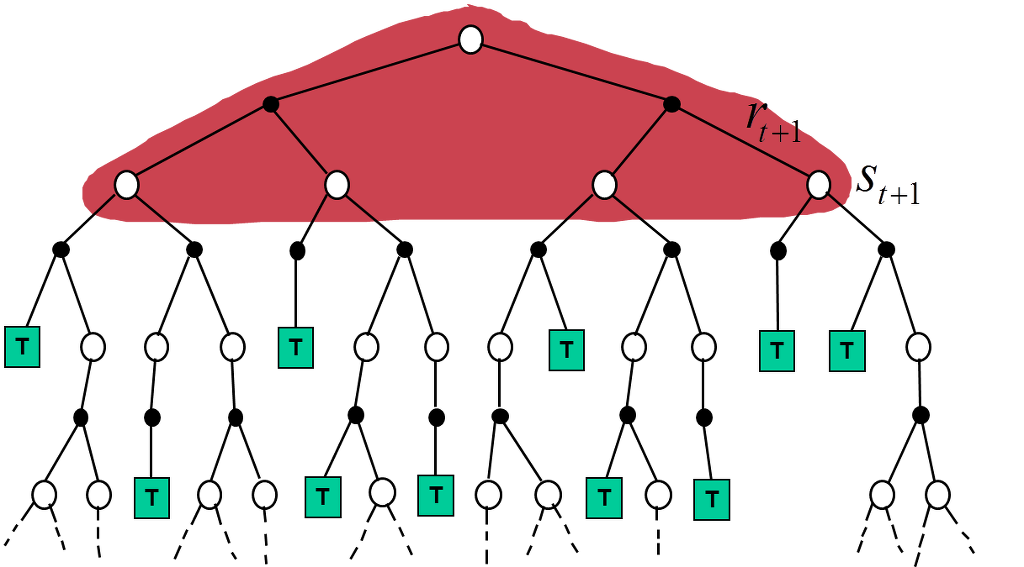
\includegraphics[width=7cm, keepaspectratio]{images/solving_10}
\end{center}
\end{column}
\end{columns}
\end{frame}

\begin{frame}{Markov döntési folyamatok dinamikus programozása}
A Markov döntési folyamatok kielégítik a dinamikus programozás feltételeit.\\
Az értékfüggvény eltárolja és újra felhasználja a kiszámított megoldásokat: ez egy gyorsítótárként szolgál azoknak az információknak az MDP-ről, ami megadja, hogy mennyi a jutalom várható értéke egy $s$ állapotból indulva:
\begin{block}{}
\[
v_{\pi}(s)=E_{\pi}\left[G_{t}|S_{t}=s\right]=E_{\pi}\left[\sum_{k=0}^{\infty}\gamma^{k}r_{t+k+1}\mid S_{t}=s\right]
\]
\end{block}
A Bellman egyenlet megadja, hogyan kell lebontani az optimális állapot-érték függvényt két részre: a következő időlépés optimális cselekvése és az összes többi lépés optimális cselekvése:\\
\begin{block}{}
\[
v_{\pi}(s)=\sum_{a}\pi(a|s)\sum_{s',r}p\left(s',r|s,a\right)\left[r+\gamma v_{\pi}\left(s'\right)\right]\;minden\;s\in S-re
\]
\end{block}
\end{frame}

\begin{frame}{Dinamikus programozás felhasználásai}
\begin{columns}
\begin{column}{.5\textwidth}
A dinamikus programozási eljárások akkor tudnak megoldani megerősítéses tanulási problémákat, ha adott a környezet dinamikája (az állapotok, az állapotátmeneti valószínűségek, jutalmak). Ezért két fő felhasználása van:\\
\begin{block}{1. Politika kiértékelés}
Ha adott egy $MDP(S,A,P,R,\gamma,s_{0})$ és egy $\pi$ politika, a feladat megtalálni $\pi$-hez tartozó $v_{\pi}$ állapot-érték függvényt ahhoz, hogy meg lehessen mondani mennyire jövedelmező a politika. 
\end{block}
\end{column}
\begin{column}{.5\textwidth}
\begin{block}{2. Politika keresés}
Ha adott egy $MDP(S,A,P,R,\gamma,s_{0})$, a feladat megtalálni az optimális állapot-érték függvényt ($v_{\pi}$) és a hozzá tartozó $\pi_{*}$ optimális politikát. 
\end{block}
\begin{center}
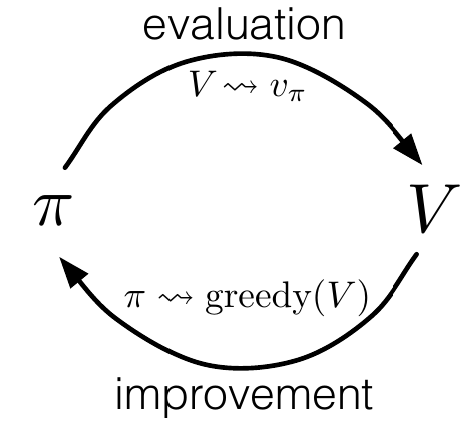
\includegraphics[width=4.5cm, keepaspectratio]{images/solving_9.png}
\end{center}
\end{column}
\end{columns}
\end{frame}

\section{Politika iteráció}

\begin{frame}
\tableofcontents[currentsection]
\end{frame}

\begin{frame}{Politika iteráció}
\begin{columns}
\begin{column}{.6\textwidth}
Miután egy $\pi$ politika javult $v_\pi$ segítségével annak érdekében, hogy egy $\pi'$ jobb politikát eredményezzen ki lehet számítani $v_{\pi'}$ javított állapot-érték függvényt és felhasználni egy újabb javított politika, $\pi''$ kiszámítására. Ezáltal egy monoton javuló politika - értékfüggvény sorozatot eredményezve:
\begin{small}
\[
\pi_{0}\stackrel{E}{\longrightarrow}v_{\pi_{0}}\stackrel{I}{\longrightarrow}\pi_{1}\stackrel{E}{\longrightarrow}v_{\pi_{1}}\stackrel{I}{\longrightarrow}\pi_{2}\stackrel{E}{\longrightarrow}\hdots\stackrel{I}{\longrightarrow}\pi_{*}\stackrel{E}{\longrightarrow}v_{*}
\]
\begin{itemize}
	\item $E$: Kiértékelés (evaluation)\\
	\item $I$: Javítás (improvement)
	\item $v_{*}$: Optimális állapot-érték függvény
	\item $\pi_{*}$: Optimális politika
\end{itemize}
\end{small}
\end{column}
\begin{column}{.4\textwidth}
\begin{center}
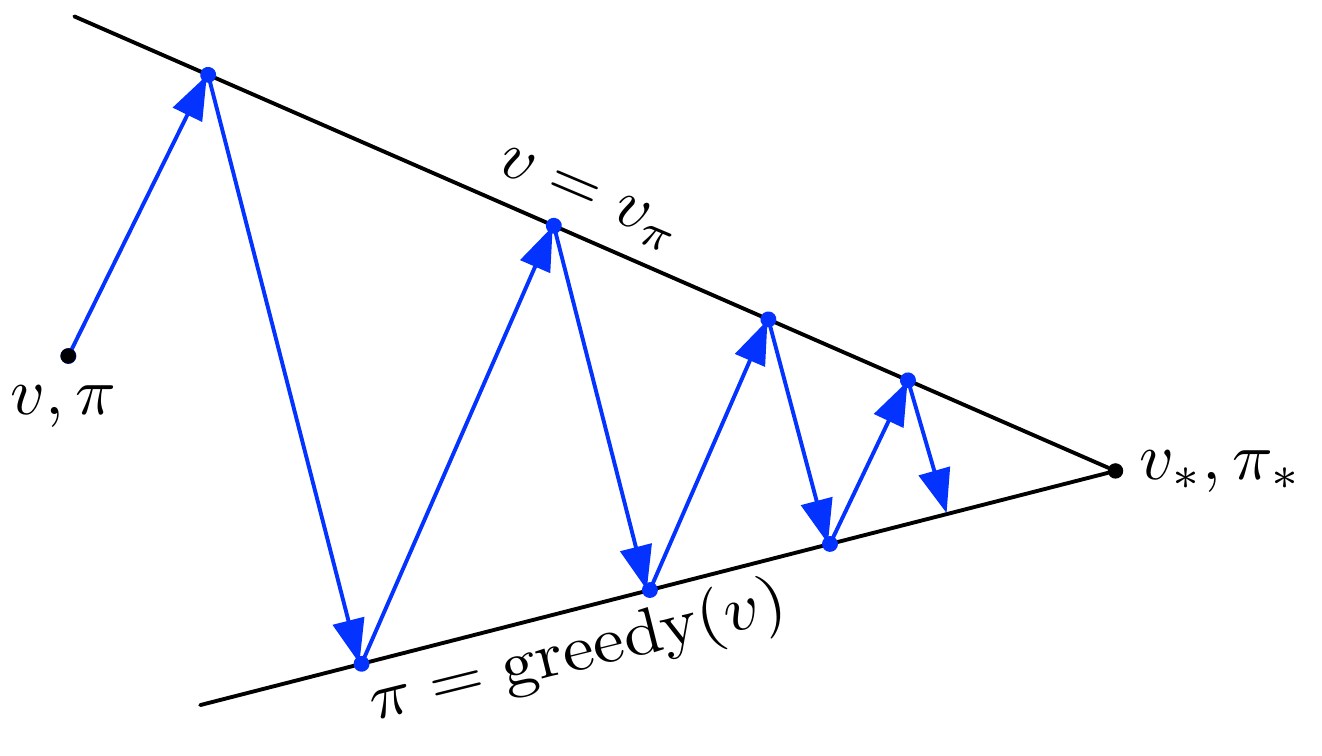
\includegraphics[width=6cm, keepaspectratio]{images/solving_11.png}
\end{center}
\end{column}
\end{columns}
\end{frame}

\begin{frame}
\begin{algorithm}[H]
\caption{Politika kiértékelése}
\SetAlgoLined
	\While{$\Delta > \theta$}{
		$\Delta \leftarrow 0$\tcc*[t]{Hiba nullára állítása}
		\For{$s \in S$}{
			$v \leftarrow V(s)$\tcc*[t]{Jelenlegi állapot-érték}
			$V(s)\leftarrow\sum_{s',r}p\left(s',r,|s,\pi(s)\right)\left[r+\gamma V(s')\right]$\tcc*[t]{Új állapot-érték}
			$\Delta \leftarrow max(\Delta, |v-V(s)|)$\tcc*[t]{Hiba kiszámolása}
		}
	}
\end{algorithm}
\begin{itemize}
	\item $\Delta$: $V(s)$ jelen állapot-érték és $V(s_{t+1})$ következő állapot-érték különbsége.
	\item $\theta$: hibahatár: egy alacsony szám ami a becslés pontosságát adja.
	\item $p\left(s',r,|s,\pi(s)\right)$: $s'$ következő állapot és $r$ jutalom valószínűsége ha adott $s$ állapot és $\pi(s)$ cselekvés $\pi$ politika szerint (a környezet dinamikája).
\end{itemize}
\end{frame}

\begin{frame}
\begin{algorithm}[H]
\caption{Politika javítása}
\SetAlgoLined
	$\pi_{instabil} \leftarrow\; false$\tcc*[t]{Politika instabilon indul}
	\While{$\pi_{instabil}$}{
		\For{$s \in S$}{
			$a \leftarrow \pi(s)$\tcc*[t]{Jelenlegi cselekvés}
			$\pi(s) \leftarrow \underset{a}{argmax}\sum_{s',r}p\left(s',r,|s,a\right)\left[r+\gamma V(s')\right]$\tcc*[t]{Új cselekvés}
			\If{$a \neq \pi(s)$}{
				$\pi_{instabil} \leftarrow\; false$\tcc*[t]{politika instabillá állítása}
			}		
		}
	}
	return $v \thickapprox v_{*}$, $\pi \thickapprox \pi_{*}$
\end{algorithm}
A politika ebben az esetben mohó, tehát úgy választja ki a cselekvést, hogy melyik következő állapothoz tartozik a lehető legnagyobb várható jutalom. Egy politika akkor számít stabilnak, amikor egyik lépésben sem változik a cselekvés. 
\end{frame}

\begin{frame}{Példa politika iterációra}
\begin{columns}
\begin{column}{.8\textwidth}
Cél: a robotnak el kell jutnia a célhoz, miközben minél kevesebb üzemanyagot használ. A környezetben a következő változók érvényesek:
\begin{itemize}
	\item Száraz kockák:	
	\begin{itemize}
		\item $1$ időegység alatt megy végig rajta a robot. $-1$ jutalmat kap ha egy ilyen kockára lép.
		\item A célállapotot mindig eléri, mert ilyenkor nem csúszik el.
	\end{itemize}		
	\item Kis tócsák:
	\begin{itemize}
		\item $2$ időegység rajta átjutni, tehát $-2$ jutalmat kap érte a robot.
		\item A csúszás valószínűsége $0.4$, ezért az idő $40\%$-ában nem éri el a célállapotot, hanem valamelyik másik lehetséges célállapotba csúszik át.
	\end{itemize}
	\item Nagy tócsák:
	\begin{itemize}
		\item $4$ időegység alatt lehet rajta átjutni, ezért $-4$ jutalom jár érte.
		\item A csúszás valószínűsége $0.6$.
	\end{itemize}
\end{itemize}
\end{column}
\begin{column}{.2\textwidth}
\begin{center}
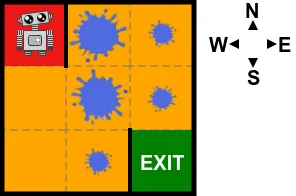
\includegraphics[width=3cm, keepaspectratio]{images/solving_12.png}
\vspace{1cm}
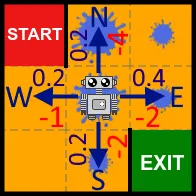
\includegraphics[width=3cm, keepaspectratio]{images/solving_13.png}
\end{center}
\end{column}
\end{columns}
\end{frame}

\begin{frame}{Példa politika iterációra}
\only<1>{\begin{center}
A robotnak a bal felső kockából kell a jobb alsóba eljutnia úgy, hogy a falakat megkerüli.\\
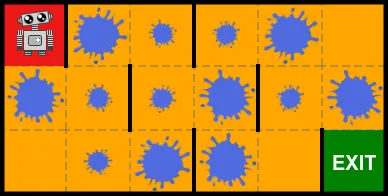
\includegraphics[width=7cm, keepaspectratio]{images/policy_iteration_0.png}
\end{center}}
\only<2>{\begin{center}
A kezdeti politika véletlenszerű és determinisztikus.\\
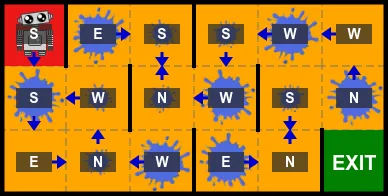
\includegraphics[width=7cm, keepaspectratio]{images/policy_iteration_1.png}
\end{center}}
\only<3>{\begin{center}
A $V(s)$ állapot értékek $0$ értékkel indulnak.\\
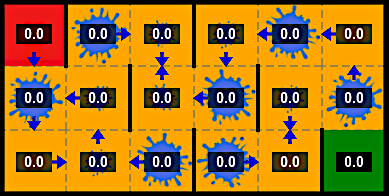
\includegraphics[width=7cm, keepaspectratio]{images/policy_iteration_2.png}
\end{center}}
\only<4>{\begin{center}
$\gamma=0.9$ diszkont rátával a politika kiértékelés $75$ iteráció alatt konvergál.\\
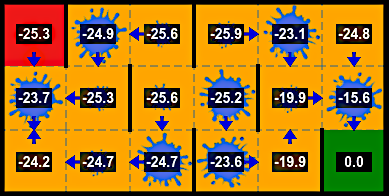
\includegraphics[width=7cm, keepaspectratio]{images/policy_iteration_3.png}
\end{center}}
\only<5>{\begin{center}
A következő iterációban a politika változik. A konvergálás $55$ iteráció alatt megtörtént.\\
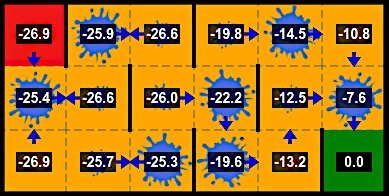
\includegraphics[width=7cm, keepaspectratio]{images/policy_iteration_4.png}
\end{center}}
\only<6>{\begin{center}
A következő futtatással $26$ iteráció alatt konvergált.\\
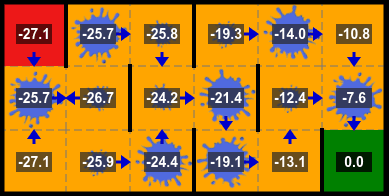
\includegraphics[width=7cm, keepaspectratio]{images/policy_iteration_5.png}
\end{center}}
\only<7>{\begin{center}
A következő futtatással $21$ iteráció alatt konvergált.\\
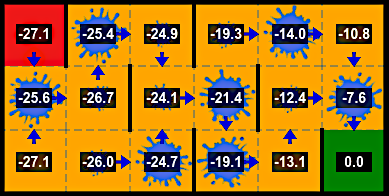
\includegraphics[width=7cm, keepaspectratio]{images/policy_iteration_6.png}
\end{center}}
\only<8>{\begin{center}
A következő futtatással $26$ iteráció alatt konvergált.\\
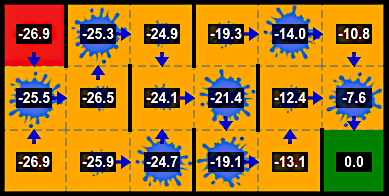
\includegraphics[width=7cm, keepaspectratio]{images/policy_iteration_7.png}
\end{center}}
\end{frame}

\end{document}












